%-------------------------------------------------------
% SLEPc Users Manual
%-------------------------------------------------------
\chapter{\label{cap:int}Getting Started}
%-------------------------------------------------------

\noindent \slepc, the {\em Scalable Library for Eigenvalue Problem Computations}, is a software library for the solution of large sparse eigenvalue problems on parallel computers.

	Together with linear systems of equations, eigenvalue problems are a very important class of linear algebra problems. The need for the numerical solution of these problems arises in many situations in science and engineering, in problems associated with stability and vibration analysis in practical applications. These are usually formulated as large sparse eigenproblems.

	Computing eigenvalues is essentially more difficult than solving linear systems of equations. This has resulted in a very active research activity in the area of computational methods for eigenvalue problems in the last years, with many remarkable achievements.  However, these state-of-the-art methods and algorithms are not easily transferred to the scientific community, and, apart from a few exceptions, most user still rely on simpler, well-established techniques.
	
	The reasons for this situation are diverse. First, new methods are increasingly complex and difficult to implement and therefore robust implementations must be provided by computational specialists, for example as software libraries. The development of such libraries requires to invest a lot of effort but sometimes they do not reach normal users due to a lack of awareness.
	
	In the case of eigenproblems, using libraries is not straightforward. It is usually recommended that the user understands how the underlying algorithm works and typically the problem is successfully solved only after several cycles of testing and parameter tuning. Methods are often specific for a certain class of eigenproblems and this leads to an explosion of available algorithms from which the user has to choose. Not all these algorithms are available in the form of software libraries, even less frequently with parallel capabilities.
	
	Another difficulty resides in how to represent the operator matrix. Unlike in dense methods, there is no widely accepted standard for basic sparse operations in the spirit of \blas. This is due to the fact that sparse storage is more complicated, admitting of more variation, and therefore less standardized. For this reason, sparse libraries have an added level of complexity. This holds even more so in the case of parallel distributed-memory programming, where the data of the problem have to be distributed across the available processors.
	
	The first implementations of algorithms for sparse matrices required a prescribed storage format for the sparse matrix, which is an obvious limitation. An alternative way of matrix representation is by means of a user-provided subroutine for the matrix-vector product. Apart from being format-independent, this approach allows the solution of problems in which the matrix is not available explicitly. The drawback is the restriction to a fixed-prototype subroutine.

	A better solution for the matrix representation problem is the well-known reverse communication interface, a technique that allows the development of iterative methods disregarding the implementation details of various operations. Whenever the iterative method subroutine needs the results of one of the operations, it returns control to the user's subroutine that called it. The user's subroutine then invokes the module that performs the operation. The iterative method subroutine is invoked again with the results of the operation.

	Several libraries with any of the interface schemes mentioned above are publicly available. For a survey of such software see the \slepc Technical Report \hyperlink{str}{[STR-6]}, ``A Survey of Software for Sparse Eigenvalue Problems'', and references therein. Some of the most recent libraries are even prepared for parallel execution (some of them can be used from within \slepc, see \S\ref{sec:wrap}). However, they still lack some flexibility or require too much programming effort from the user, especially in the case that the eigensolution requires to employ advanced techniques such as spectral transformations or preconditioning.

	A further obstacle appears when these libraries have to be used in the context of large software projects carried out by inter-disciplinary teams. In this scenery, libraries must be able to interoperate with already existing software and with other libraries. In order to cope with the complexity associated with such projects, libraries must be designed carefully in order to overcome hurdles such as different storage formats or programming languages. In the case of parallel software, care must be taken also to achieve portability to a wide range of platforms with good performance and still retain flexibility and usability.

%---------------------------------------------------
\section{SLEPc and PETSc}

	The \slepc library is an attempt to provide a solution to the situation described in the previous paragraphs. It is intended to be a general library for the solution of eigenvalue problems that arise in different contexts, covering standard and generalized problems, both Hermitian and non-Hermitian, with either real or complex arithmetic. Issues such as usability, portability, efficiency and interoperability are addressed, and special emphasis is put on flexibility, providing data-structure neutral implementations and multitude of run-time options. \slepc offers a growing number of eigensolvers as well as interfaces to integrate well-established eigenvalue packages such as \arpack. In addition to the linear eigenvalue problem, \slepc also includes other solver classes for nonlinear eigenproblems, SVD and the computation of the action of a matrix function.

	\slepc is based on \petsc, the Portable, Extensible Toolkit for Scientific Computation \citep{Balay:PUM}, and, therefore, a large percentage of the software complexity is avoided since many \petsc developments are leveraged, including matrix storage formats and linear solvers, to name a few. \slepc focuses on high level features for eigenproblems, structured around a few object classes as described below.

	\petsc uses modern programming paradigms to ease the development of large-scale scientific application codes in Fortran, C, and C++ and provides a powerful set of tools for the numerical solution of partial differential equations and related problems on high-performance computers. Its approach is to encapsulate mathematical algorithms using object-oriented programming techniques, which allow to manage the complexity of efficient numerical message-passing codes. All the \petsc software is free and used around the world in a variety of application areas.

	The design philosophy is not to try to completely conceal parallelism from the application programmer. Rather, the user initiates a combination of sequential and parallel phases of computations, but the library handles the detailed message passing required during the coordination of computations. Some of the design principles are described in \citep{Balay:1997:EMP}.

	\petsc is built around a variety of data structures and algorithmic objects. The application programmer works directly with these objects rather than concentrating on the underlying data structures. Each component manipulates a particular family of objects (for instance, vectors) and the operations one would like to perform on the objects. The three basic abstract data objects are index sets, vectors and matrices. Built on top of this foundation are various classes of solver objects, which encapsulate virtually all information regarding the solution procedure for a particular class of problems, including the local state and various options such as convergence tolerances, etc.

	\slepc can be considered an extension of \petsc providing all the functionality necessary for the solution of eigenvalue problems. Figure \ref{fig:slepc} shows a diagram of all the different objects included in \petsc (on the left) and those added by \slepc (on the right). \petsc is a prerequisite for \slepc and users should be familiar with basic concepts such as vectors and matrices in order to use \slepc. Therefore, together with this manual we recommend to use the \petsc Users Manual \citep{Balay:PUM}.

\begin{figure}[t]
\centering
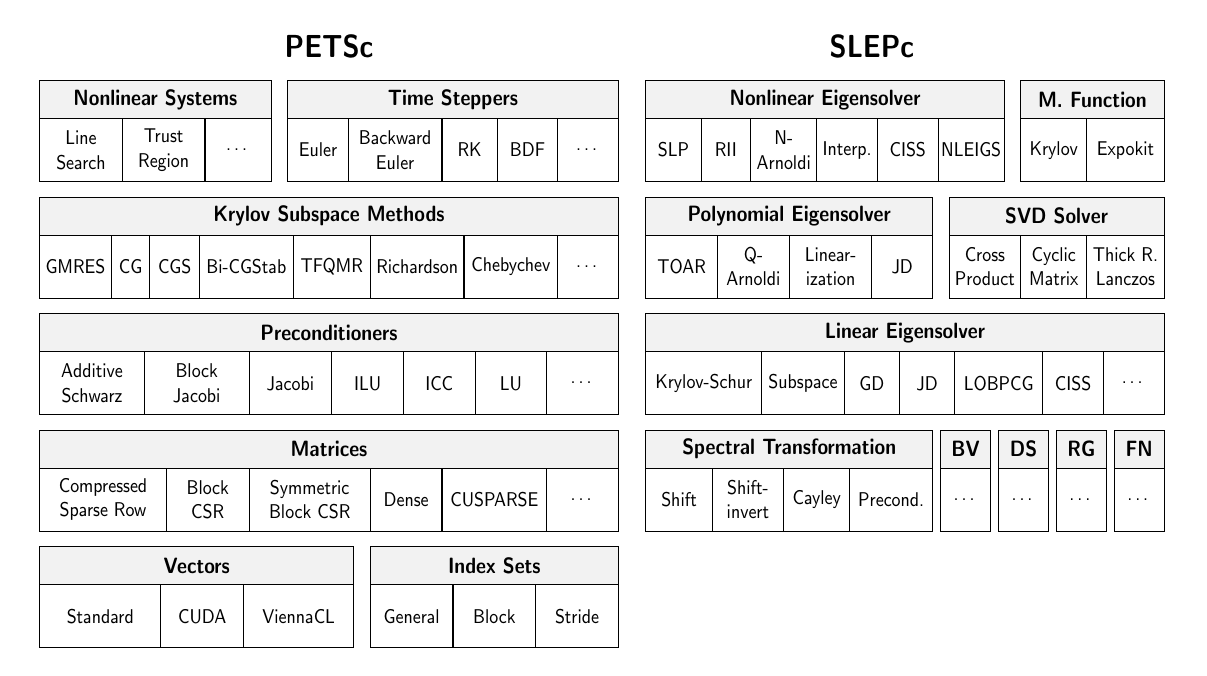
\begin{tikzpicture}[xscale=0.7,yscale=0.8]
  \tikzstyle{interface}=[fill=black!5,font=\sffamily\bfseries]
  \tikzstyle{implem}=[font=\sffamily\small,text badly centered]
  \tikzstyle{every node}=[transform shape]
  \def\levsep{1.85} % separation of levels
  \def\hint{0.6} % height interface
  \def\himp{1} % height implementation
  \node[above,text centered,font=\sffamily\bfseries\Large] at (5.25,5*\levsep) {PETSc};
  \draw[interface] (0,\himp) rectangle node {Vectors} +(5.7,\hint);
  \draw[implem] (0,0) rectangle node {Standard} ++(2.2,1) ++(0,-1)
                      rectangle node {CUDA} ++(1.5,1) ++(0,-1)
                      rectangle node {ViennaCL} ++(2.0,1);
  \draw[interface] (6,\himp) rectangle node {Index Sets} +(4.5,\hint);
  \draw[implem] (6,0) rectangle node {General} ++(1.5,1) ++(0,-1)
                rectangle node {Block} ++(1.5,1) ++(0,-1)
                rectangle node {Stride} ++(1.5,1);
  \draw[interface] (0,\levsep+\himp) rectangle node {Matrices} +(10.5,\hint);
  \draw[implem] (0,\levsep) rectangle node[text width=2.5cm] {Compressed Sparse Row} ++(2.3,1) ++(0,-1)
                rectangle node[text width=1.3cm] {Block CSR} ++(1.5,1) ++(0,-1)
                rectangle node[text width=2.3cm] {Symmetric Block CSR} ++(2.2,1) ++(0,-1)
                rectangle node {Dense} ++(1.3,1) ++(0,-1)
                rectangle node {CUSPARSE} ++(1.9,1) ++(0,-1)
                rectangle node {\dots} ++(1.3,1);
  \draw[interface] (0,2*\levsep+\himp) rectangle node {Preconditioners} +(10.5,\hint);
  \draw[implem] (0,2*\levsep) rectangle node[text width=1.7cm] {Additive Schwarz} ++(1.9,1) ++(0,-1)
                rectangle node[text width=1.7cm] {Block Jacobi} ++(1.9,1) ++(0,-1)
                rectangle node {Jacobi} ++(1.5,1) ++(0,-1)
                rectangle node {ILU} ++(1.3,1) ++(0,-1)
                rectangle node {ICC} ++(1.3,1) ++(0,-1)
                rectangle node {LU} ++(1.3,1) ++(0,-1)
                rectangle node {\dots} ++(1.3,1);
  \draw[interface] (0,3*\levsep+\himp) rectangle node {Krylov Subspace Methods} +(10.5,\hint);
  \draw[implem] (0,3*\levsep) rectangle node {GMRES} ++(1.3,1) ++(0,-1)
                rectangle node {CG} ++(0.7,1) ++(0,-1)
                rectangle node {CGS} ++(0.9,1) ++(0,-1)
                rectangle node {Bi-CGStab} ++(1.7,1) ++(0,-1)
                rectangle node {TFQMR} ++(1.4,1) ++(0,-1)
                rectangle node {Richardson} ++(1.7,1) ++(0,-1)
                rectangle node {Chebychev} ++(1.7,1) ++(0,-1)
                rectangle node {\dots} ++(1.1,1);
  \draw[interface] (0,4*\levsep+\himp) rectangle node {Nonlinear Systems} +(4.2,\hint);
  \draw[implem] (0,4*\levsep) rectangle node[text width=1.2cm] {Line Search} ++(1.5,1) ++(0,-1)
                rectangle node[text width=1.2cm] {Trust Region} ++(1.5,1) ++(0,-1)
                rectangle node {\dots} ++(1.2,1);
  \draw[interface] (4.5,4*\levsep+\himp) rectangle node {Time Steppers} +(6,\hint);
  \draw[implem] (4.5,4*\levsep) rectangle node {Euler} ++(1.1,1) ++(0,-1)
                rectangle node[text width=1.5cm] {Backward Euler} ++(1.7,1) ++(0,-1)
                rectangle node[text width=1.8cm] {RK} ++(1.0,1) ++(0,-1)
                rectangle node[text width=1.8cm] {BDF} ++(1.1,1) ++(0,-1)
                rectangle node {\dots} ++(1.1,1);
  \node[above,text centered,font=\sffamily\bfseries\Large] at (15.1,5*\levsep) {SLEPc};
  \draw[interface] (11,4*\levsep+\himp) rectangle node {Nonlinear Eigensolver} +(6.5,\hint);
  \draw[implem] (11,4*\levsep) rectangle node {SLP} ++(1,1) ++(0,-1)
                rectangle node {RII} ++(.9,1) ++(0,-1)
                rectangle node[text width=1.2cm] {N\-Arnoldi} ++(1.2,1) ++(0,-1)
                rectangle node[text width=1.2cm] {Interp.} ++(1.1,1) ++(0,-1)
                rectangle node {CISS} ++(1.1,1) ++(0,-1)
                rectangle node[text width=1.2cm] {NLEIGS} ++(1.2,1);
  \draw[interface] (17.8,4*\levsep+\himp) rectangle node {M.~Function} +(2.6,\hint);
  \draw[implem] (17.8,4*\levsep) rectangle node {Krylov} ++(1.2,1) ++(0,-1)
                rectangle node {Expokit} ++(1.4,1);
  \draw[interface] (11,3*\levsep+\himp) rectangle node {Polynomial Eigensolver} +(5.2,\hint);
  \draw[implem] (11,3*\levsep) rectangle node[text width=1.2cm] {TOAR} ++(1.3,1) ++(0,-1)
                rectangle node[text width=1.2cm] {Q\-Arnoldi} ++(1.3,1) ++(0,-1)
                rectangle node[text width=1.7cm] {Linear\-ization} ++(1.5,1) ++(0,-1)
                rectangle node {JD} ++(1.1,1) ++(0,-1);
  \draw[interface] (16.5,3*\levsep+\himp) rectangle node {SVD Solver} +(3.9,\hint);
  \draw[implem] (16.5,3*\levsep) rectangle node[text width=1.2cm] {Cross Product} ++(1.3,1) ++(0,-1)
                rectangle node[text width=1.2cm] {Cyclic Matrix} ++(1.2,1) ++(0,-1)
                %rectangle node {Lanczos} ++(1.3,1) ++(0,-1)
                rectangle node[text width=1.7cm] {Thick R. Lanczos} ++(1.4,1);
  \draw[interface] (11,2*\levsep+\himp) rectangle node {Linear Eigensolver} +(9.4,\hint);
  \draw[implem] (11,2*\levsep) rectangle node {Krylov-Schur} ++(2.1,1) ++(0,-1)
                rectangle node {Subspace} ++(1.5,1) ++(0,-1)
                rectangle node {GD} ++(1.0,1) ++(0,-1)
                rectangle node {JD} ++(1.0,1) ++(0,-1)
                rectangle node {LOBPCG} ++(1.6,1) ++(0,-1)
                rectangle node {CISS} ++(1.1,1) ++(0,-1)
                rectangle node {\dots} ++(1.1,1);
  \draw[interface] (11,\levsep+\himp) rectangle node {Spectral Transformation} +(5.2,\hint);
  \draw[implem] (11,\levsep) rectangle node {Shift} ++(1.2,1) ++(0,-1)
                rectangle node[text width=1.5cm] {Shift-invert} ++(1.3,1) ++(0,-1)
                rectangle node {Cayley} ++(1.2,1) ++(0,-1)
                rectangle node {Precond.} ++(1.5,1);
  \draw[interface] (16.35,\levsep+\himp) rectangle node {BV} +(.9,\hint) ++(1.05,0)
                   rectangle node {DS} +(.9,\hint) ++(1.05,0)
                   rectangle node {RG} +(.9,\hint) ++(1.05,0)
                   rectangle node {FN} +(.9,\hint);
  \draw[implem] (16.35,\levsep) rectangle node {\dots} ++(.9,1);
  \draw[implem] (17.4,\levsep) rectangle node {\dots} ++(.9,1);
  \draw[implem] (18.45,\levsep) rectangle node {\dots} ++(.9,1);
  \draw[implem] (19.5,\levsep) rectangle node {\dots} ++(.9,1);
\end{tikzpicture}
\caption{\label{fig:slepc}Numerical components of \petsc and \slepc.}
\end{figure}

	Each of these components consists of an abstract interface (simply a set of calling sequences) and one or more implementations using particular data structures. Both \petsc and \slepc are written in C, which lacks direct support for object-oriented programming. However, it is still possible to take advantage of the three basic principles of object-oriented programming to manage the complexity of such large packages. \petsc uses data \emph{encapsulation} in both vector and matrix data objects. Application code accesses data through function calls. Also, all the operations are supported through \emph{polymorphism}. The user calls a generic interface routine, which then selects the underlying routine that handles the particular data structure. Finally, \petsc also uses \emph{inheritance} in its design. All the objects are derived from an abstract base object. From this fundamental object, an abstract base object is defined for each \petsc\ object (\texttt{Mat}, \texttt{Vec} and so on), which in turn has a variety of instantiations that, for example, implement different matrix storage formats.

	\petsc/\slepc provide clean and effective codes for the various phases of solving PDEs, with a uniform approach for each class of problems.  This design enables easy comparison and use of different algorithms (for example, to experiment with different Krylov subspace methods, preconditioners, or eigensolvers). Hence, \petsc, together with \slepc, provides a rich environment for modeling scientific applications as well as for rapid algorithm design and prototyping.

	Options can be specified by means of calls to subroutines in the source code and also as command-line arguments. Runtime options allow the user to test different tolerances, for example, without having to recompile the program. Also, since \petsc provides a uniform interface to all of its linear solvers ---the Conjugate Gradient, GMRES, etc.--- and a large family of preconditioners ---block Jacobi, overlapping additive Schwarz, etc.---, one can compare several combinations of method and preconditioner by simply specifying them at execution time. \slepc shares this good property.
	
	The components enable easy customization and extension of both algorithms and implementations. This approach promotes code reuse and flexibility, and separates the issues of parallelism from the choice of algorithms.  The \petsc infrastructure creates a foundation for building large-scale applications.

%---------------------------------------------------
\section{Installation}
\label{sec:inst}

	This section describes \slepc's installation procedure.
	Previously to the installation of \slepc, the system must have an appropriate version of \petsc\ installed. Compatible versions of \petsc and \slepc are those with coincident major and minor version number, the third number (patch level) being irrelevant for this. For instance, \slepc 3.17.x may be built with \petsc 3.17.x. Also note that, if using git repositories, both \petsc and \slepc must be either release versions or development versions, so make sure you select the appropriate branch in both repositories (\texttt{git checkout release} or \texttt{git checkout main}).

	The installation process for \slepc is very similar to \petsc, with two stages: configuration and compilation. \slepc's configuration is much simpler because most of the configuration information is taken from \petsc, including compiler options and scalar type (real or complex). See \S\ref{sec:opt-inst} for a discussion of options that are most relevant for \slepc. Several configurations can coexist in the same directory tree, so that for instance one can have \slepc libraries compiled with real scalars as well as with complex scalars. This is explained in \S\ref{sec:mult-inst}. Also, system-based installation is also possible with the \Verb!--prefix! option, as discussed in \S\ref{sec:prefix-inst}.

\subsection{Standard Installation}
\label{sec:std-inst}

	The basic steps for the installation are described next. Note that prior to these steps, optional packages must have been installed. If any of these packages is installed afterwards, reconfiguration and recompilation is necessary. Refer to \S\ref{sec:opt-inst} and \S\ref{sec:wrap} for details about installation of some of these packages.

\begin{enumerate}
	\item Unbundle the distribution file with
	\begin{Verbatim}[fontsize=\small]
	$ tar xzf slepc-3.17.0.tar.gz
	\end{Verbatim}
        or an equivalent command. This will create a directory and unpack the software there.
	\item Set the environment variable \ident{SLEPC\_DIR} to the full path of the \slepc home directory. For example, under the \texttt{bash} shell:
	\begin{Verbatim}[fontsize=\small]
	$ export SLEPC_DIR=/home/username/slepc-3.17.0
	\end{Verbatim}
	In addition, the variables \ident{PETSC\_DIR} and \ident{PETSC\_ARCH} must also be set appropriately, e.g.
	\begin{Verbatim}[fontsize=\small]
	$ export PETSC_DIR=/home/username/petsc-3.17.0
	$ export PETSC_ARCH=arch-darwin-c-debug
	\end{Verbatim}
        The rationale for \ident{PETSC\_ARCH} is explained in \S\ref{sec:mult-inst} (see \S\ref{sec:prefix-inst} for a case in which \ident{PETSC\_ARCH} is not required).
	\item\label{step-config} Change to the \slepc directory and run the configuration script:
	\begin{Verbatim}[fontsize=\small]
	$ cd $SLEPC_DIR
	$ ./configure
	\end{Verbatim}
	\item If the configuration was successful, build the libraries:
	\begin{Verbatim}[fontsize=\small]
	$ make
	\end{Verbatim}
	\item After the compilation, try running some test examples with
	\begin{Verbatim}[fontsize=\small]
	$ make check
	\end{Verbatim}
        Examine the output for any obvious errors or problems.
\end{enumerate}
	
\subsection{Configuration Options}
\label{sec:opt-inst}

Several options are available in \slepc's configuration script. To see all available options, type \Verb!./configure --help!.

In \slepc, configure options have the following purposes:
\begin{itemize}
%\item Build \slepc with Python interfaces, as explained in \S\ref{sec:py-inst}.
\item Specify a directory for prefix-based installation, as explained in \S\ref{sec:prefix-inst}.
\item Enable external eigensolver packages. For example, to use \arpack, specify the following options (with the appropriate paths):
	\begin{Verbatim}[fontsize=\small]
	$ ./configure --with-arpack-dir=/usr/software/ARPACK
	\end{Verbatim}
Some of the external packages also support the \Verb!--download-xxxx! option. Section \ref{sec:wrap} provides more details related to use of external libraries.
\end{itemize}

Additionally, \petsc's configuration script provides a very long list of options that are relevant to \slepc. Here is a list of options that may be useful. Note that these are options of \petsc that apply to both \petsc and \slepc, in such a way that it is not possible to, e.g., build \petsc without debugging and \slepc with debugging.
\begin{itemize}
\item Add \Verb!--with-scalar-type=complex! to build complex scalar versions of all libraries. See below a note related to complex scalars.
\item Build single precision versions with \Verb!--with-precision=single!. In most applications, this can achieve a significant reduction of memory requirements, and a moderate reduction of computing time. Also, quadruple precision (128-bit floating-point representation) is also available using \Verb!--with-precision=__float128! on systems with GNU compilers (\texttt{gcc-4.6} or later).
\item Enable use from Fortran. By default, \petsc's configure looks for an appropriate Fortran compiler. If not required, this can be disabled: \Verb!--with-fc=0!. If required but not correctly detected, the compiler to be used can be specified with a configure option. It is also possible to configure with a Fortran compiler but do not build Fortran interfaces of \petsc and \slepc, with \Verb!--with-fortran-bindings=0!.
\item If not detected, use \Verb!--with-blas-lapack-lib! to specify the location of \blas and \lapack. If \slepc's configure complains about some missing \lapack subroutines, reconfigure \petsc with option \Verb!--download-f2cblaslapack!.
\item Enable external libraries that provide direct linear solvers or preconditioners, such as MUMPS, hypre, or SuperLU; for example, \Verb!--download-mumps!. These are especially relevant for \slepc in the case that a spectral transformation is used, see chapter \ref{cap:st}.
\item Add \Verb!--with-64-bit-indices=1! to use 8 byte integers (\texttt{long long}) for indexing in vectors and matrices. This is only needed when working with over roughly 2 billion unknowns.
\item Build static libraries, \Verb!--with-shared-libraries=0!. This is generally not recommended, since shared libraries produce smaller executables and the run time overhead is small.
\item Error-checking code can be disabled with \Verb!--with-debugging=0!, but this is only recommended in production runs of well-tested applications.
\item Enable GPU computing setting \Verb!--with-cuda=1!; see \S\ref{sec:gpu} for details.
\item The option \Verb!--with-mpi=0! allows building \petsc and \slepc without MPI support (only sequential).
\end{itemize}

\medskip
\textbf{Note about complex scalar versions}: \petsc supports the use of complex scalars by defining the data type \ident{PetscScalar} either as a real or complex number. This implies that two different versions of the \petsc libraries can be built separately, one for real numbers and one for complex numbers, but they cannot be used at the same time. \slepc inherits this property. In \slepc it is not possible to completely separate real numbers and complex numbers because the solution of non-symmetric real-valued eigenvalue problems may be complex. \slepc has been designed trying to provide a uniform interface to manage all the possible cases. However, there are slight differences between the interface in each of the two versions. In this manual, differences are clearly identified.

\subsection{Installing Multiple Configurations in a Single Directory Tree}
\label{sec:mult-inst}

Often, it is necessary to build two (or more) versions of the libraries that differ in a few configuration options. For instance, versions for real and complex scalars, or versions for double and single precision, or versions with debugging and optimized. In a standard installation, this is handled by building all versions in the same directory tree, as explained below, so that source code is not replicated unnecessarily. In contrast, in prefix-based installation where source code is not present, the issue of multiple configurations is handled differently, as explained in \S\ref{sec:prefix-inst}.

In a standard installation, the different configurations are identified by a unique name that is assigned to the environment variable \ident{PETSC\_ARCH}. Let us illustrate how to set up \petsc with two configurations. First, set a value of \ident{PETSC\_ARCH} and proceed with the installation of the first one:
	\begin{Verbatim}[fontsize=\small]
	$ cd $PETSC_DIR
	$ export PETSC_ARCH=arch-linux-gnu-c-debug-real
	$ ./configure --with-scalar-type=real
	$ make all
	\end{Verbatim}
Note that if \ident{PETSC\_ARCH} is not given a value, \petsc suggests one for us. After this, a subdirectory named \texttt{\$PETSC\_ARCH} is created within \texttt{\$PETSC\_DIR}, that stores all information associated with that configuration, including the built libraries, configuration files, automatically generated source files, and log files. For the second configuration, proceed similarly:
	\begin{Verbatim}[fontsize=\small]
	$ cd $PETSC_DIR
	$ export PETSC_ARCH=arch-linux-gnu-c-debug-complex
	$ ./configure --with-scalar-type=complex
	$ make all
	\end{Verbatim}
The value of \ident{PETSC\_ARCH} in this case must be different than the previous one. It is better to set the value of \ident{PETSC\_ARCH} explicitly, because the name suggested by \texttt{configure} may coincide with an existing value, thus overwriting a previous configuration. After successful installation of the second configuration, two \texttt{\$PETSC\_ARCH} directories exist within \texttt{\$PETSC\_DIR}, and the user can easily choose to build his/her application with either configuration by simply changing the value of \ident{PETSC\_ARCH}.

The configuration of two versions of \slepc in the same directory tree is very similar. The only important restriction is that the value of \ident{PETSC\_ARCH} used in \slepc must exactly match an existing \petsc configuration, that is, a directory \texttt{\$PETSC\_DIR/\$PETSC\_ARCH} must exist.

\subsection{Prefix-based Installation}
\label{sec:prefix-inst}

Both \petsc and \slepc allow for prefix-based installation. This consists in specifying a directory to which the files generated during the building process are to be copied.

In \petsc, if an installation directory has been specified during configuration (with option \Verb!--prefix! in step \ref{step-config} of \S\ref{sec:std-inst}), then after building the libraries the relevant files are copied to that directory by typing
	\begin{Verbatim}[fontsize=\small]
	$ make install
	\end{Verbatim}
	This is useful for building as a regular user and then copying the libraries and include files to the system directories as root.

To be more precise, suppose that the configuration was done with \texttt{-{}-prefix=/opt/petsc-3.17.0-linux-gnu-c-debug}. Then, \texttt{make install} will create directory \texttt{/opt/petsc-3.17.0-linux-gnu-c-debug} if it does not exist, and several subdirectories containing the libraries, the configuration files, and the header files. Note that the source code files are not copied, nor the documentation, so the size of the installed directory will be much smaller than the original one. For that reason, it is no longer necessary to allow for several configurations to share a directory tree. In other words, in a prefix-based installation, variable \ident{PETSC\_ARCH} loses significance and must be unset. To maintain several configurations, one should specify different prefix directories, typically with a name that informs about the configuration options used.

In order to prepare a prefix-based installation of \slepc that uses a prefix-based installation of \petsc, start by setting the appropriate value of \ident{PETSC\_DIR}. Then, run \slepc's configure with a prefix directory.
	\begin{Verbatim}[fontsize=\small,numbers=none]
	$ export PETSC_DIR=/opt/petsc-3.17.0-linux-gnu-c-debug
	$ unset PETSC_ARCH
	$ cd $SLEPC_DIR
	$ ./configure --prefix=/opt/slepc-3.17.0-linux-gnu-c-debug
	$ make
	$ make install
	$ export SLEPC_DIR=/opt/slepc-3.17.0-linux-gnu-c-debug
	\end{Verbatim}
Note that the variable \ident{PETSC\_ARCH} has been unset before \slepc's configure. \slepc will use a temporary arch name during the build (this temporary arch is named \texttt{installed-arch-xxx}, where the \texttt{arch-xxx} string represents the configuration of the installed \petsc version). Although it is not a common case, it is also possible to configure \slepc without prefix, in which case the \ident{PETSC\_ARCH} variable must still be empty and the arch directory \texttt{installed-xxx} is picked automatically (it is hardwired in file \texttt{\$SLEPC\_DIR/lib/slepc/conf/slepcvariables}). The combination \petsc without prefix and \slepc with prefix is also allowed, in which case \ident{PETSC\_ARCH} should not be unset.

%\subsection{Building Python Interfaces}
%\label{sec:py-inst}

%---------------------------------------------------
\section{Running SLEPc Programs}

Before using \slepc, the user must first set the environment variable
\ident{SLEPC\_DIR}, indicating the full path of the directory containing \slepc. For example, under the \texttt{bash} shell, a command of the form
	\begin{Verbatim}[fontsize=\small]
	$ export SLEPC_DIR=/software/slepc-3.17.0
	\end{Verbatim}
can be placed in the user's \Verb!.bashrc! file.
The \ident{SLEPC\_DIR} directory can be either a standard installation \slepc directory, or a prefix-based installation directory, see \S\ref{sec:prefix-inst}.
In addition, the user must set the environment variables required by \petsc, that is, \ident{PETSC\_DIR}, to indicate the full path of the \petsc directory, and \ident{PETSC\_ARCH} to specify a particular architecture and set of options. Note that \ident{PETSC\_ARCH} should not be set in the case of prefix-based installations.

All \petsc programs use the MPI (Message Passing Interface) standard
for message-passing communication \citep{MPI-Forum:1994:MMI}.  Thus, to execute
\slepc programs, users must know the procedure for launching MPI jobs
on their selected computer system(s).  Usually, the \texttt{mpiexec} command can be used to initiate a program as in the following example that uses eight processes:
	\begin{Verbatim}[fontsize=\small]
	$ mpiexec -n 8 slepc_program [command-line options]
	\end{Verbatim}
Note that MPI may be deactivated during configuration of \petsc, if one wants to run only serial programs in a laptop, for example.

All \petsc-compliant programs support the use of the \Verb!-h!
or \Verb!-help! option as well as the \Verb!-v! or \Verb!-version! option. In the case of \slepc programs, specific information for \slepc is also displayed.

%---------------------------------------------------
\section{Writing SLEPc Programs}

	Most \slepc programs begin with a call to \rutina{SlepcInitialize}
	\begin{Verbatim}[fontsize=\small]
	SlepcInitialize(int *argc,char ***argv,char *file,char *help);
	\end{Verbatim}
which initializes \slepc, \petsc and MPI. This subroutine is very similar to \rutina{PetscInitialize}, and the arguments have the same meaning. In fact, internally \rutina{SlepcInitialize} calls \rutina{PetscInitialize}.

	After this initialization, \slepc programs can use communicators defined by \petsc. In most cases users can employ the communicator \ident{PETSC\_COMM\_WORLD} to indicate all processes in a given run and \ident{PETSC\_COMM\_SELF} to indicate a single process. MPI provides routines for generating new communicators consisting of subsets of processes, though most users rarely need to use these features. \slepc users need not program much message passing directly with MPI, but they must be familiar with the basic concepts of message passing and distributed memory computing.

	All \slepc programs should call \rutina{SlepcFinalize} as their final (or nearly final) statement
	\begin{Verbatim}[fontsize=\small]
	SlepcFinalize();
	\end{Verbatim}
This routine handles operations to be executed at the conclusion of the program, and calls \rutina{PetscFinalize} if \rutina{SlepcInitialize} began \petsc.

\medskip
\textbf{Note to Fortran Programmers}: In this manual all the examples and calling sequences are given for the C/C++ programming languages. However, Fortran programmers can use most of the functionality of \slepc and \petsc from Fortran, with only minor differences in the user interface. For instance, the two functions mentioned above have their corresponding Fortran equivalent:
	\begin{Verbatim}[fontsize=\small]
	call SlepcInitialize(file,ierr)
	call SlepcFinalize(ierr)
	\end{Verbatim}
Section \ref{sec:fortran} provides a summary of the differences between using \slepc from Fortran and C/C++, as well as a complete Fortran example.

%---------------------------------------------------
\subsection{Simple SLEPc Example}
\label{sec:simpleex}

	A simple example is listed next that solves an eigenvalue problem associated with the one-dimensional Laplacian operator discretized with finite differences. This example can be found in \Verb!${SLEPC_DIR}/src/eps/tutorials/ex1.c!. Following the code we highlight a few of the most important parts of this example.

\MyVerbatimInput{ex1.c}

\paragraph{Include Files.}

The C/C++ include files for \slepc should be used via statements such as
	\begin{Verbatim}[fontsize=\small]
	#include <slepceps.h>
	\end{Verbatim}
where \Verb!slepceps.h! is the include file for the \ident{EPS} component. Each \slepc program must specify an include file that corresponds to the highest level \slepc objects needed within the program; all of the required lower level include files are automatically included within the higher level files. For example, \Verb!slepceps.h! includes \Verb!slepcst.h! (spectral transformations), and \Verb!slepcsys.h! (base \slepc file). Some \petsc header files are included as well, such as \Verb!petscksp.h!. The \slepc include files are located in the directory \Verb!${SLEPC_DIR}/include!.

\paragraph{The Options Database.}

All the \petsc functionality related to the options database is available in \slepc. This allows the user to input control data at run time very easily. In this example, the call \Verb!PetscOptionsGetInt(NULL,NULL,"-n",&n,NULL)! checks whether the user has provided a command line option to set the value of \Verb!n!, the problem dimension.  If so, the variable \Verb!n! is set accordingly; otherwise, \Verb!n! remains unchanged.

\paragraph{Vectors and Matrices.}

Usage of matrices and vectors in \slepc is exactly the same as in \petsc. The user can create a new parallel or sequential matrix, \texttt{A}, which has \texttt{M} global rows and \texttt{N} global columns, with
	\begin{Verbatim}[fontsize=\small]
	MatCreate(MPI_Comm comm,Mat *A);
	MatSetSizes(Mat A,PetscInt m,PetscInt n,PetscInt M,PetscInt N);
	MatSetFromOptions(Mat A);
	MatSetUp(Mat A);
	\end{Verbatim}
where the matrix format can be specified at runtime. The example creates a matrix, sets the nonzero values with \rutina{MatSetValues} and then assembles it.

\paragraph{Eigensolvers.}

Usage of eigensolvers is very similar to other kinds of solvers provided by \petsc. After creating the matrix (or matrices) that define the problem, $Ax = kx$ (or $Ax=kBx$), the user can then use \ident{EPS} to solve the system with the following sequence of commands:
\findex{EPSCreate} \findex{EPSSetOperators} \findex{EPSSetProblemType}
\findex{EPSSetFromOptions} \findex{EPSSolve} \findex{EPSDestroy}
\findex{EPSGetConverged} \findex{EPSGetEigenpair}
	\begin{Verbatim}[fontsize=\small,numbers=none]
	EPSCreate(MPI_Comm comm,EPS *eps);
	EPSSetOperators(EPS eps,Mat A,Mat B);
        EPSSetProblemType(EPS eps,EPSProblemType type);
	EPSSetFromOptions(EPS eps);
	EPSSolve(EPS eps);
	EPSGetConverged(EPS eps,PetscInt *nconv);
	EPSGetEigenpair(EPS eps,PetscInt i,PetscScalar *kr,PetscScalar *ki,Vec xr,Vec xi);
	EPSDestroy(EPS *eps);
	\end{Verbatim}
The user first creates the \ident{EPS} context and sets the operators associated with the eigensystem as well as the problem type. The user then sets various options for customized solution, solves the problem, retrieves the solution, and finally destroys the \ident{EPS} context. Chapter~\ref{cap:eps} describes in detail the \ident{EPS} package, including
the options database that enables the user to customize the solution process at runtime by selecting the solution algorithm and also specifying the convergence tolerance, the number of eigenvalues, the dimension of the subspace, etc.

\paragraph{Spectral Transformation.}

In the example program shown above there is no explicit reference to spectral transformations. However, an \ident{ST} object is handled internally so that the user is able to request different transformations such as shift-and-invert. Chapter~\ref{cap:st} describes the \ident{ST} package in detail.

\paragraph{Error Checking.}

	All \slepc routines return an integer indicating whether an error has occurred during the call. The error code is set to be nonzero if an error has been detected; otherwise, it is zero. The \petsc macro \Verb!PetscCall(...)! checks the return value and calls the \petsc error handler upon error detection. \Verb!PetscCall(...)! should be used in all subroutine calls to enable a complete error traceback. See the \petsc documentation for full details.

\subsection{Writing Application Codes with SLEPc}

Several example programs demonstrate the software usage and can serve as templates for developing custom applications. They are scattered throughout the \slepc directory tree, in particular in the \Verb!tutorials! directories under each class subdirectory.

To write a new application program using \slepc, we suggest the following procedure:
\begin{enumerate}
\item Install and test \slepc according to the instructions given in the documentation.
\item Copy the \slepc example that corresponds to the class of problem of interest (e.g., singular value decomposition).
\item Create a makefile as explained below, compile and run the example program.
\item Use the example program as a starting point for developing a custom code.
\end{enumerate}

	Application program makefiles can be set up very easily just by including one file from the \slepc makefile system. All the necessary \petsc{} definitions are loaded automatically. The following sample makefile illustrates how to build C and Fortran programs:

	\begin{Verbatim}[fontsize=\small]
default: ex1

include ${SLEPC_DIR}/lib/slepc/conf/slepc_common

ex1: ex1.o
	-${CLINKER} -o ex1 ex1.o ${SLEPC_EPS_LIB}
	${RM} ex1.o

ex1f: ex1f.o
	-${FLINKER} -o ex1f ex1f.o ${SLEPC_EPS_LIB}
	${RM} ex1f.o
	\end{Verbatim}

